\chapter{Proposed Methodology}
This chapter describes the methodology of the Phase-I system. Section~4.1 presents the adaptive planning loop that ties the four components together. Section~4.2 states the candidate models considered for each component and the model selected for the delivered system. Section~4.3 describes the offline comparison methodology used to make that selection. Section~4.4 records how the system design evolved during development, from a predict-then-optimize scheduler to a capacity-based booking model. Section~4.5 describes the resulting system architecture and the split between client-side and server-side computation.

\section{The Adaptive Planning Loop}
The planner is organised as an open loop over the learner's own logged sessions. A session is logged, the learner's pace is recalibrated from the accumulated history, the pace series is checked for a behavioural shift, the completion date is re-projected, and the schedule is regenerated when the projection diverges from the deadline. The loop is deliberately open rather than automatic: a detected shift raises a recalibration prompt, and the learner decides whether to replan. This keeps the learner in control of a plan that is theirs, and it avoids acting on a shift that the learner knows to be a one-off. Figure~\ref{fig:loop} shows the four components and the signal that passes between them.

\begin{figure}[htbp]
\centering
\resizebox{\linewidth}{!}{%
\begin{tikzpicture}[node distance=6mm and 10mm, font=\small, >=Latex,
  lstep/.style={draw, rounded corners=3pt, line width=0.8pt, align=center, inner sep=5pt, text width=2.5cm, fill=blue!4},
  io/.style={draw, rounded corners=10pt, line width=0.8pt, align=center, inner sep=5pt, text width=2.3cm, fill=black!4}]
\node[io] (S) {Logged sessions};
\node[lstep, right=of S] (C) {Pace calibration};
\node[lstep, right=of C] (D) {Change detection};
\node[lstep, right=of D] (P) {Progress projection};
\node[lstep, right=of P] (R) {Schedule regeneration};
\draw[->] (S) -- (C);
\draw[->] (C) -- (D);
\draw[->] (D) -- (P);
\draw[->] (P) -- (R);
\draw[->] (R.south) -- ++(0,-0.8) -| node[pos=0.25, below, font=\scriptsize, fill=white, inner sep=1.5pt]{updated plan shapes future sessions} (S.south);
\node[font=\scriptsize, text=black!60, align=center] at ($(D)!0.5!(P)+(0,1.15)$) {recalibration prompt\\(learner decides)};
\draw[->, dashed, draw=black!45] ($(D.north)+(0,0.05)$) to[out=90,in=90] ($(R.north)+(0,0.05)$);
\end{tikzpicture}%
}
\caption{The open adaptive loop. Logged sessions drive pace calibration, change detection, and progress projection; a detected shift raises a recalibration prompt, and the learner decides whether to regenerate the schedule, which in turn shapes future sessions.}
\label{fig:loop}
\end{figure}

\section{Candidate Models and Selected Approach}
Each component was chosen by comparing candidate models offline rather than by assumption. This section states the candidates and the selected model; Section~4.3 describes how the comparison was run. Table~\ref{tab:candidates} summarises the choices.

\subsection{Pace Calibration}
The calibration candidates were a simple moving average of the pace ratio, an exponentially weighted moving average, a pooled Bayesian estimate, and the hierarchical Bayesian model of Equation~\eqref{eq:bayes-update}. Under rigorous held-out evaluation the structured candidates did not beat the hierarchical Bayesian baseline, which is reported honestly in Chapter~6. The model that did improve on the baseline is a context-aware shrinkage calibrator developed for this project. Let $\phi_t \in \mathbb{R}^d$ be a vector of observable context features for session $t$, covering the material role, the time of day, the day of week, proximity to the deadline, planned progress, and recency, and let $y_t = \log(a_t/p_t)$ be the log pace ratio. The calibrator fits weights $w$ by ridge-regularised least squares shrunk toward a population prior $w_0$ rather than toward zero,
\begin{equation}
\hat{w} = \arg\min_{w}\ \sum_t \big(y_t - w^{\top}\phi_t\big)^2 \; + \; \lambda\,\lVert w \rVert^2 \; + \; \gamma\,\lVert w - w_0 \rVert^2,
\label{eq:enriched}
\end{equation}
where $\lambda$ is the ridge strength and $\gamma$ the shrinkage strength, both fixed at values validated offline. The pace multiplier for a context $\phi$ is $\exp(\hat{w}^{\top}\phi)$. Shrinking toward a population prior makes the model behave sensibly when a learner has logged few sessions and converge to learner-specific behaviour as sessions accumulate. The delivered calibrator is an ensemble of two such models seeded with different population priors and combined by leave-one-out-weighted averaging.

\subsection{Change Detection}
The detection candidates were the one-sided CUSUM chart of Equation~\eqref{eq:cusum}, an exponentially weighted moving-average control chart, a critical-slowing-down detector, the Page-Hinkley test, Bayesian online change-point detection, and ADWIN. The delivered system uses the single-arm CUSUM. As Chapter~6 reports, the comparison is a robust null: no candidate improves on the established CUSUM and critical-slowing-down frontier, and CUSUM is the fastest detector, which suits raising a human-confirmed recalibration prompt.

\subsection{Progress Projection}
The projection candidates were linear extrapolation of cumulative progress, Gaussian-process regression under the kernel of Equation~\eqref{eq:gp-kernel}, a composite that falls back to an analytic estimate when the learner has too few sessions for the Gaussian process to be trusted, and a split-conformal correction of the interval width. The delivered system uses the Gaussian process with the cold-start composite, which was validated as an improvement on the plain Gaussian process for low-data plans. The split-conformal interval correction is recorded in Chapter~6 as a validated refinement not yet shipped.

\subsection{Schedule Generation}
The scheduling candidates were a rule-based baseline, a dynamic-programming capacity allocator of the form in Equation~\eqref{eq:dp}, a greedy prerequisite-aware packer, and a local-search repair heuristic. On the synthetic data the dynamic-programming allocator minimised deadline drift. The delivered system does not use it. As Section~4.4 records, the day-by-day packing formulation these candidates share proved brittle in practice and worked against continuous replanning, so the system was redesigned around a capacity-based booking model. Scheduling is therefore reported in Chapter~6 as an evaluated component whose result informed a design decision, not as a shipped optimiser.

\begin{table}[htbp]
\centering
\footnotesize
\caption{Candidate models per component and the model selected for the delivered Phase-I system.}
\label{tab:candidates}
\begin{tabular}{p{2.6cm} p{6.2cm} p{3.4cm}}
\toprule
\textbf{Component} & \textbf{Candidates compared} & \textbf{Selected (delivered)} \\
\midrule
Pace calibration & Moving average, EWMA, pooled Bayesian, hierarchical Bayesian, context-aware shrinkage & Hierarchical Bayesian with the context-aware shrinkage calibrator \\
Change detection & CUSUM, EWMA control chart, critical slowing down, Page-Hinkley, Bayesian online change-point, ADWIN & Single-arm CUSUM (robust null: nothing beats the CUSUM/CSD frontier) \\
Progress projection & Linear extrapolation, Gaussian process, GP with cold-start composite, split-conformal correction & Gaussian process with the cold-start composite \\
Schedule generation & Rule-based, dynamic-programming capacity, greedy prerequisite-aware, local-search repair & None shipped; replaced by capacity-based booking (Section~4.4) \\
\bottomrule
\end{tabular}
\end{table}

\section{Comparison Methodology}
The comparison rests on synthetic data with known ground truth, so that each component can be scored against a truth that real learner logs do not provide. A synthetic generator produces study histories in which the learner's true pace, the timing and size of any regime shift, and the completion behaviour are planted and therefore known. The generator's parameters were calibrated against a large public learning-management-system dataset so that the synthetic regime resembles observed learner behaviour rather than an arbitrary one. Candidate models are evaluated on held-out learner archetypes that are absent from the set used to develop them, so that a win reflects generalisation rather than fitting to the evaluation cases. Figure~\ref{fig:pipeline} shows the pipeline.

\begin{figure}[htbp]
\centering
\resizebox{\linewidth}{!}{%
\begin{tikzpicture}[node distance=5mm and 9mm, font=\small, >=Latex,
  b/.style={draw, rounded corners=3pt, line width=0.8pt, align=center, inner sep=5pt, text width=2.6cm, fill=black!3}]
\node[b] (G) {Synthetic generator\\\scriptsize (known ground truth)};
\node[b, right=of G] (M) {Candidate models\\\scriptsize run per component};
\node[b, right=of M] (E) {Per-component metrics};
\node[b, right=of E] (S) {Bootstrap CIs\\$+$ Holm/BH gate};
\node[b, right=of S] (W) {Selected model};
\draw[->] (G) -- (M); \draw[->] (M) -- (E); \draw[->] (E) -- (S); \draw[->] (S) -- (W);
\node[b, below=of M, fill=orange!12, draw=black!40] (O) {Oracle\\\scriptsize (upper-bound baseline)};
\draw[->, draw=black!45] (O) -- (E);
\end{tikzpicture}%
}
\caption{The offline comparison pipeline. The synthetic generator supplies ground truth; each candidate is scored on per-component metrics; a bootstrap confidence interval and Holm/Benjamini--Hochberg correction gate the result before a model is selected. The oracle is an upper-bound reference, not a deployable method.}
\label{fig:pipeline}
\end{figure}

Each component is scored on metrics appropriate to it, defined in Table~\ref{tab:metrics}. Every reported comparison carries a bootstrap confidence interval on the difference between a candidate and the incumbent, and a Holm or Benjamini--Hochberg correction is applied across the family of comparisons so that a win survives multiple-comparison scrutiny. An oracle baseline, which is given the planted ground truth, is included as an upper bound on achievable performance; it is a reference ceiling and is never treated as a deployable method.

\begin{table}[htbp]
\centering
\footnotesize
\caption{Evaluation metrics by component.}
\label{tab:metrics}
\begin{tabular}{p{3.0cm} p{9.0cm}}
\toprule
\textbf{Component} & \textbf{Metrics} \\
\midrule
Pace calibration & Mean absolute error of the recovered pace against the planted pace \\
Change detection & Detection latency after a planted shift, and the false-alarm rate \\
Progress projection & Coverage of the 95\% interval against nominal, and point error in days \\
Schedule generation & Deadline drift and the number of capacity violations \\
\bottomrule
\end{tabular}
\end{table}

\section{System Design and Evolution}
The system did not arrive at its current shape in one step, and the path is worth recording because it explains why the delivered scheduler differs from the one the comparison favoured.

The starting point was the predict-then-optimize architecture of the base paper~\cite{islam2024}, in which a predictive model estimates the learner's pace and an optimizer turns the estimate into a schedule. The initial design realised this literally. The intelligence service ran calibration, detection, projection, and a constraint-based schedule generator, and the generator packed each material onto a specific calendar day, producing the dated slot grid shown in Figure~\ref{fig:arch-initial}. A replan re-ran the packer on the service and returned a new grid.

\begin{figure}[htbp]
\centering
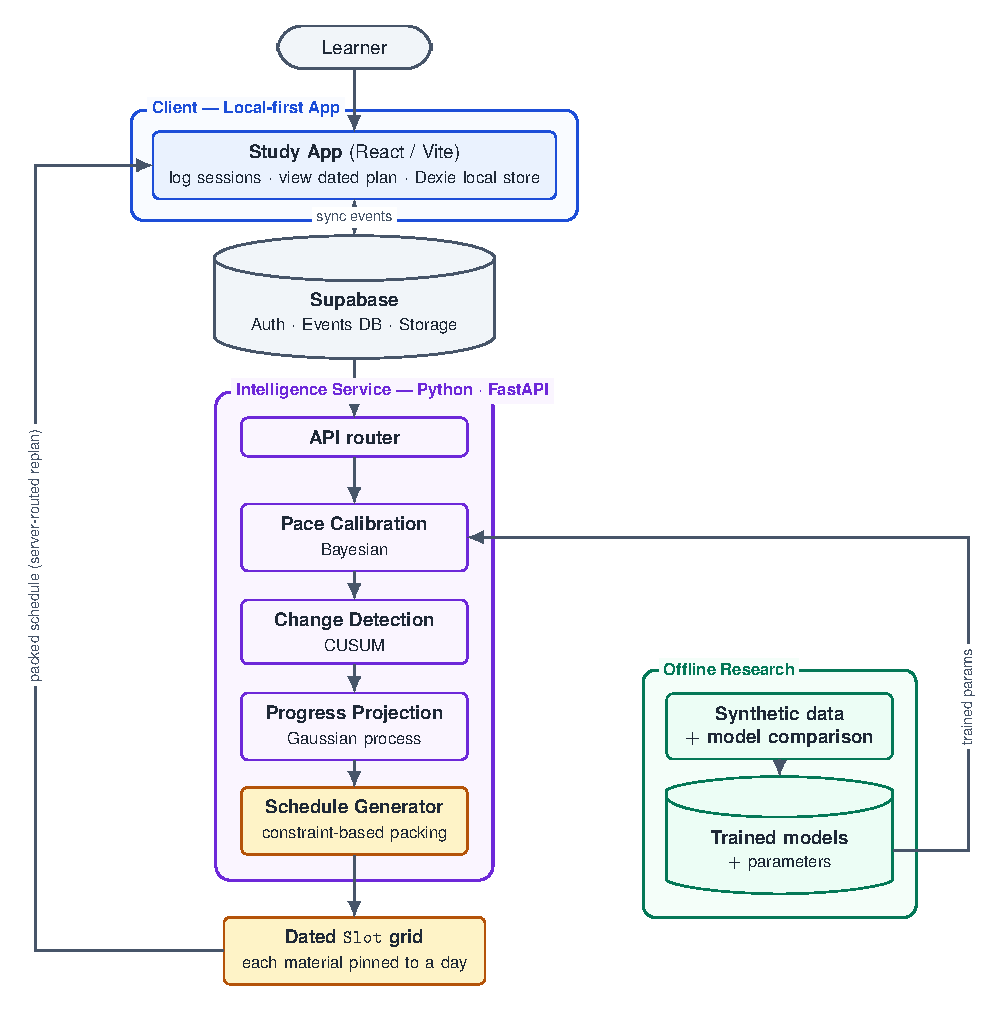
\includegraphics[width=0.66\textwidth]{arch_initial.pdf}
\caption{Initial design (predict-then-optimize). The intelligence service runs all four components, and the schedule generator packs each material onto a fixed day, returning a dated \texttt{Slot} grid; a replan re-runs the packer on the service.}
\label{fig:arch-initial}
\end{figure}

This design proved brittle in use. Pinning materials to fixed days created boundary and tie cases at the edges of the packing that were awkward to resolve, and the rigid day-by-day grid worked against the central goal of continuous replanning: every change to the learner's pace forced a re-pack of the whole grid. The problem the packer solved, deciding exactly which material to study on which day, was also not the problem the learner actually had, which was knowing whether they were on track and what to do next.

The design was therefore revised. The scheduling question was re-examined on a revised synthetic regime that models the new interaction pattern, and the calibration, detection, and projection models were confirmed to transfer to it. The prescriptive packer was retired in favour of a capacity-based booking model: the plan holds blank bookings, each carrying a date and a duration, and the learner picks a material at the start of a session. The engine's job shrinks from packing a grid to estimating a capacity and projecting a finish date. Figure~\ref{fig:arch-revised} shows the resulting architecture.

\begin{figure}[htbp]
\centering
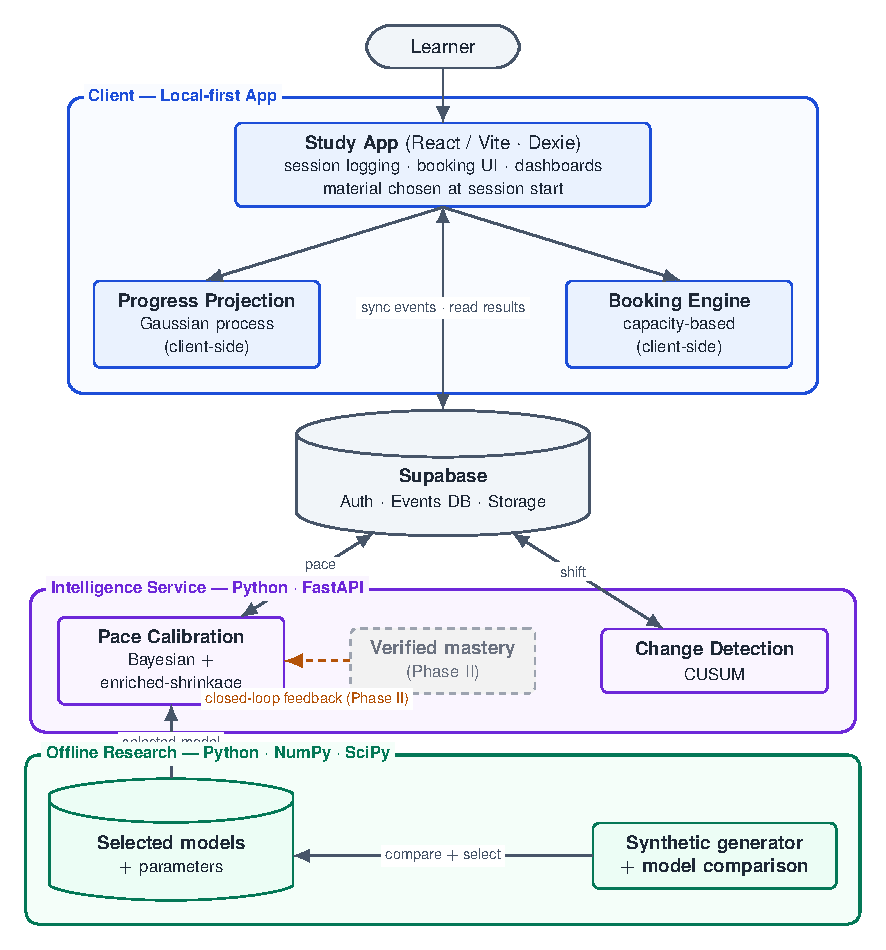
\includegraphics[width=0.74\textwidth]{arch_revised.pdf}
\caption{Revised design (capacity-based booking), the delivered system. Progress projection and the booking engine run client-side; Bayesian and enriched-shrinkage calibration and CUSUM detection run in the Python service; Supabase is the data hub; the offline research pipeline supplies the selected models. The closed-loop feedback from verified mastery is drawn dashed as Phase-II work.}
\label{fig:arch-revised}
\end{figure}

\section{System Architecture}
The delivered system is organised into three tiers, shown in Figure~\ref{fig:arch-revised}, with computation deliberately split between the client and the service according to what each part needs.

The client is a local-first single-page application built with React and Vite, storing every event in a per-user IndexedDB database through Dexie. It owns the parts of the system that derive directly from the learner's local event log: session logging, the booking user interface, the dashboards, the Gaussian-process progress projection, and the capacity-based booking engine. Running these client-side keeps the core loop responsive and available offline. The intelligence service is a Python and FastAPI application that hosts the parts that fit a statistical model to accumulated data: Bayesian and enriched-shrinkage pace calibration and CUSUM change detection. The client calls the service over HTTP, and every request carries a signed token that the service verifies before any model runs. The division follows a simple rule: computation that fits a model to history runs on the service, and computation that derives a view from the local event log runs on the client. Supabase sits between the two as the data hub, providing authentication, the event database, and object storage, with each learner's data isolated by row-level security. An offline research pipeline, described in Section~4.3, supplies the trained models and parameters that the calibrator uses. The closed-loop feedback from verified mastery back into calibration, shown dashed in Figure~\ref{fig:arch-revised}, is the principal Phase-II extension and is not part of the delivered Phase-I system.
